% !TEX root = ../../../../main/numb3rs_activities.tex
\newpage
\phantomsection
\addcontentsline{toc}{subsection}{501: High Exposure \label{ep501}}
\ep{501: High Exposure}
\setcounter{activity}{0}

In this episode, two climbers are found dead in a national 5park, one with a large high-value uncut diamond hidden in his pack. A report comes in that a diamond shipment has gone missing en route, and the team discovers that it was supposed to be delivered by a charter plane which left one airport, but never arrived at its destination. Without transponder or radar information to help determine the flight path, the possible crash area is too big to cover in the amount of time they have. The question is to determine a probabilistic flight path, that is, to narrow the search by finding the probability that the plane took that route, given a set of conditions. These constraints could include the topography of the land, weather conditions, and whether the pilot wanted to minimize distance or take the scenic route.


Let us take our map and overlay a grid, and just consider paths along the edges of the grid as a model. For each vertex, labeled by a letter and a number, we assign a probability to each edge leaving the vertex.


\begin{itemize}
\item If we sum all the edges leaving a vertex, what should they add up to? Why?

	\begin{figure}[H]
	\centering
	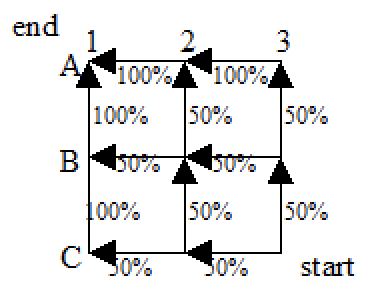
\includegraphics[width=0.30\textwidth]{../sections/seasons/season5/501/images/cover_me.png}
	\end{figure}

\end{itemize}


To get the probability of a given path, we take the product of the probabilities of each step.


\begin{ex}
Consider the path $C3 \to C2 \to C1 \to B1 \to A1$. Then the probability that the plane took the path is
	\[
	\begin{split}
	P_{C3 \to C2 \to C1 \to B1 \to A1}&= P_{C3 \to C2} \cdot P_{C2 \to C1} \cdot P_{C1 \to B1} \cdot P_{B1 \cdot A1} \\
	&= 0.50 \cdot 0.50 \cdot 1. \cdot 1.0 \\
	&= 0.25,
	\end{split}
	\]
so that there is a 25\% probability that the plane took this path. 
\end{ex}


\begin{itemize}
\item For each of the following paths, calculate the probability that the plane took that route:
\end{itemize}


	\begin{table}[H]
	\centering
	\begin{tabular}{c}
	$C3 \to C2 \to B2 \to B1 \to A1$ \\
	$C3 \to C2 \to B2 \to A2 \to A1$ \\
	$C3 \to B3 \to B2 \to B1 \to A1$ \\
	$C3 \to B3 \to B2 \to A2 \to A1$ \\
	$C3 \to B3 \to A3 \to A2 \to A1$ \\
	\end{tabular}
	\end{table}


\begin{itemize}
\item Assume that we know the plane arrived, that it made it to A1. Then there were 6 possible paths that it could have followed. What is the probability that the plane is at A1?
\item What can you guess this means about the sum of the probabilities of all the possible routes? Check your answer.
\item Let us think mathematically about why this would be true: Assuming that we know the plane landed at its destination, what is the probability of it being at A1?
\end{itemize}


Let us generalize this to say that the probability of the plane passing through a given point is the sum of the probabilities of all the paths leading to that point.


\begin{itemize}
\item What is the probability that the plane passed through C2? B3? If we knew that the plane had only flown one distance unit, where would we want to start our search?
\item What is the probability that the plane passed through B2? C1? A3? If we knew that the plane had flown two distance units, where would we want to start our search?
\item Repeat the question for 3 distance units.
\item Repeat the question for 4 distance units.
\item In the episode, the team had no information about how long the plane was in the air. Assuming there is an equal probability that the plane went 1,2, or 3 distance units, what is the location with the highest probability overall?
\end{itemize}


In the show, the team actually has even more information. Before going missing, the climbers had talked about a great new cliff they had found. The team has a topographical map from the U.S. Geological Survey, and together with the climbers’ location and reasonable hiking distance, they can narrow down where this new cliff might be. If they can narrow down the path that the plane took, then they have a better chance of finding it, along with hopefully more evidence that will lead them to the killers.


Now let us incorporate more information into our model. Let us say that at the time the plane left the airport, there was a thunderstorm at C1, so moving in the direction of that vertex is less desirable. Maybe we also read off the USGS map that the land around A3 is mostly flat and probably does not have any great climbing cliffs. While this wouldn’t necessarily have been a factor in the pilot’s choice, we know that he went down near a great climbing cliff and therefore his path would be less probable in that region. Note that the choices are no longer symmetric!


	\begin{figure}
	\centering
	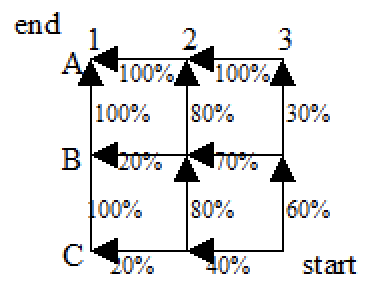
\includegraphics[width=0.3\textwidth]{../sections/seasons/season5/501/images/high_exposure.png}
	\end{figure}


\begin{itemize}
\item Repeat the above exercise to determine where the plane most likely went down in this scenario.
\end{itemize}


We can see that the more information about the situation we have, the better our model is and the better our guesses. This is important when we have finite resources, like only a few field agents able to cover the terrain, not enough helicopters, and limited search time. We also have to balance the number of grid lines with the information we have---if we have more grid lines, we can better localize our probabilities, but it might be harder to determine what those probabilities might be.